\documentclass[1p]{elsarticle_modified}
%\bibliographystyle{elsarticle-num}

%\usepackage[colorlinks]{hyperref}
%\usepackage{abbrmath_seonhwa} %\Abb, \Ascr, \Acal ,\Abf, \Afrak
\usepackage{amsfonts}
\usepackage{amssymb}
\usepackage{amsmath}
\usepackage{amsthm}
\usepackage{scalefnt}
\usepackage{amsbsy}
\usepackage{kotex}
\usepackage{caption}
\usepackage{subfig}
\usepackage{color}
\usepackage{graphicx}
\usepackage{xcolor} %% white, black, red, green, blue, cyan, magenta, yellow
\usepackage{float}
\usepackage{setspace}
\usepackage{hyperref}

\usepackage{tikz}
\usetikzlibrary{arrows}

\usepackage{multirow}
\usepackage{array} % fixed length table
\usepackage{hhline}

%%%%%%%%%%%%%%%%%%%%%
\makeatletter
\renewcommand*\env@matrix[1][\arraystretch]{%
	\edef\arraystretch{#1}%
	\hskip -\arraycolsep
	\let\@ifnextchar\new@ifnextchar
	\array{*\c@MaxMatrixCols c}}
\makeatother %https://tex.stackexchange.com/questions/14071/how-can-i-increase-the-line-spacing-in-a-matrix
%%%%%%%%%%%%%%%

\usepackage[normalem]{ulem}

\newcommand{\msout}[1]{\ifmmode\text{\sout{\ensuremath{#1}}}\else\sout{#1}\fi}
%SOURCE: \msout is \stkout macro in https://tex.stackexchange.com/questions/20609/strikeout-in-math-mode

\newcommand{\cancel}[1]{
	\ifmmode
	{\color{red}\msout{#1}}
	\else
	{\color{red}\sout{#1}}
	\fi
}

\newcommand{\add}[1]{
	{\color{blue}\uwave{#1}}
}

\newcommand{\replace}[2]{
	\ifmmode
	{\color{red}\msout{#1}}{\color{blue}\uwave{#2}}
	\else
	{\color{red}\sout{#1}}{\color{blue}\uwave{#2}}
	\fi
}

\newcommand{\Sol}{\mathcal{S}} %segment
\newcommand{\D}{D} %diagram
\newcommand{\A}{\mathcal{A}} %arc


%%%%%%%%%%%%%%%%%%%%%%%%%%%%%5 test

\def\sl{\operatorname{\textup{SL}}(2,\Cbb)}
\def\psl{\operatorname{\textup{PSL}}(2,\Cbb)}
\def\quan{\mkern 1mu \triangleright \mkern 1mu}

\theoremstyle{definition}
\newtheorem{thm}{Theorem}[section]
\newtheorem{prop}[thm]{Proposition}
\newtheorem{lem}[thm]{Lemma}
\newtheorem{ques}[thm]{Question}
\newtheorem{cor}[thm]{Corollary}
\newtheorem{defn}[thm]{Definition}
\newtheorem{exam}[thm]{Example}
\newtheorem{rmk}[thm]{Remark}
\newtheorem{alg}[thm]{Algorithm}

\newcommand{\I}{\sqrt{-1}}
\begin{document}

%\begin{frontmatter}
%
%\title{Boundary parabolic representations of knots up to 8 crossings}
%
%%% Group authors per affiliation:
%\author{Yunhi Cho} 
%\address{Department of Mathematics, University of Seoul, Seoul, Korea}
%\ead{yhcho@uos.ac.kr}
%
%
%\author{Seonhwa Kim} %\fnref{s_kim}}
%\address{Center for Geometry and Physics, Institute for Basic Science, Pohang, 37673, Korea}
%\ead{ryeona17@ibs.re.kr}
%
%\author{Hyuk Kim}
%\address{Department of Mathematical Sciences, Seoul National University, Seoul 08826, Korea}
%\ead{hyukkim@snu.ac.kr}
%
%\author{Seokbeom Yoon}
%\address{Department of Mathematical Sciences, Seoul National University, Seoul, 08826,  Korea}
%\ead{sbyoon15@snu.ac.kr}
%
%\begin{abstract}
%We find all boundary parabolic representation of knots up to 8 crossings.
%
%\end{abstract}
%\begin{keyword}
%    \MSC[2010] 57M25 
%\end{keyword}
%
%\end{frontmatter}

%\linenumbers
%\tableofcontents
%
\newcommand\colored[1]{\textcolor{white}{\rule[-0.35ex]{0.8em}{1.4ex}}\kern-0.8em\color{red} #1}%
%\newcommand\colored[1]{\textcolor{white}{ #1}\kern-2.17ex	\textcolor{white}{ #1}\kern-1.81ex	\textcolor{white}{ #1}\kern-2.15ex\color{red}#1	}

{\Large $\underline{12n_{0064}~(K12n_{0064})}$}

\setlength{\tabcolsep}{10pt}
\renewcommand{\arraystretch}{1.6}
\vspace{1cm}\begin{tabular}{m{100pt}>{\centering\arraybackslash}m{274pt}}
\multirow{5}{120pt}{
	\centering
	\includegraphics[width=112pt]{../../../GIT/diagram.site/Diagrams/png/2153_12n_0064.png}\\
\ \ \ A knot diagram\footnotemark}&
\allowdisplaybreaks
\textbf{Linearized knot diagam} \\
\cline{2-2}
 &
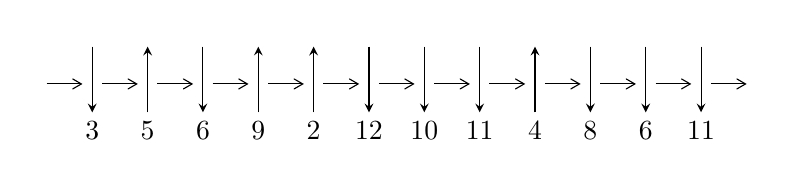
\begin{tikzpicture}[x=20pt, y=17pt]
	% nodes
	\node (C0) at (0, 0) {};
	\node (C1) at (1, 0) {};
	\node (C1U) at (1, +1) {};
	\node (C1D) at (1, -1) {3};

	\node (C2) at (2, 0) {};
	\node (C2U) at (2, +1) {};
	\node (C2D) at (2, -1) {5};

	\node (C3) at (3, 0) {};
	\node (C3U) at (3, +1) {};
	\node (C3D) at (3, -1) {6};

	\node (C4) at (4, 0) {};
	\node (C4U) at (4, +1) {};
	\node (C4D) at (4, -1) {9};

	\node (C5) at (5, 0) {};
	\node (C5U) at (5, +1) {};
	\node (C5D) at (5, -1) {2};

	\node (C6) at (6, 0) {};
	\node (C6U) at (6, +1) {};
	\node (C6D) at (6, -1) {12};

	\node (C7) at (7, 0) {};
	\node (C7U) at (7, +1) {};
	\node (C7D) at (7, -1) {10};

	\node (C8) at (8, 0) {};
	\node (C8U) at (8, +1) {};
	\node (C8D) at (8, -1) {11};

	\node (C9) at (9, 0) {};
	\node (C9U) at (9, +1) {};
	\node (C9D) at (9, -1) {4};

	\node (C10) at (10, 0) {};
	\node (C10U) at (10, +1) {};
	\node (C10D) at (10, -1) {8};

	\node (C11) at (11, 0) {};
	\node (C11U) at (11, +1) {};
	\node (C11D) at (11, -1) {6};

	\node (C12) at (12, 0) {};
	\node (C12U) at (12, +1) {};
	\node (C12D) at (12, -1) {11};
	\node (C13) at (13, 0) {};

	% arrows
	\draw[->,>={angle 60}]
	(C0) edge (C1) (C1) edge (C2) (C2) edge (C3) (C3) edge (C4) (C4) edge (C5) (C5) edge (C6) (C6) edge (C7) (C7) edge (C8) (C8) edge (C9) (C9) edge (C10) (C10) edge (C11) (C11) edge (C12) (C12) edge (C13) ;	\draw[->,>=stealth]
	(C1U) edge (C1D) (C2D) edge (C2U) (C3U) edge (C3D) (C4D) edge (C4U) (C5D) edge (C5U) (C6U) edge (C6D) (C7U) edge (C7D) (C8U) edge (C8D) (C9D) edge (C9U) (C10U) edge (C10D) (C11U) edge (C11D) (C12U) edge (C12D) ;
	\end{tikzpicture} \\
\hhline{~~} \\& 
\textbf{Solving Sequence} \\ \cline{2-2} 
 &
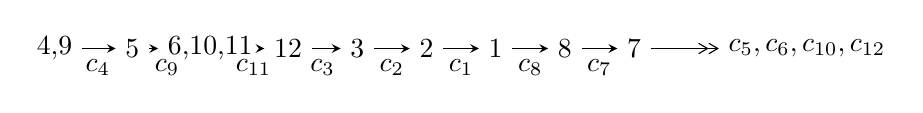
\begin{tikzpicture}[x=25pt, y=7pt]
	% node
	\node (A0) at (-1/8, 0) {4,9};
	\node (A1) at (1, 0) {5};
	\node (A2) at (17/8, 0) {6,10,11};
	\node (A3) at (13/4, 0) {12};
	\node (A4) at (17/4, 0) {3};
	\node (A5) at (21/4, 0) {2};
	\node (A6) at (25/4, 0) {1};
	\node (A7) at (29/4, 0) {8};
	\node (A8) at (33/4, 0) {7};
	\node (C1) at (1/2, -1) {$c_{4}$};
	\node (C2) at (3/2, -1) {$c_{9}$};
	\node (C3) at (11/4, -1) {$c_{11}$};
	\node (C4) at (15/4, -1) {$c_{3}$};
	\node (C5) at (19/4, -1) {$c_{2}$};
	\node (C6) at (23/4, -1) {$c_{1}$};
	\node (C7) at (27/4, -1) {$c_{8}$};
	\node (C8) at (31/4, -1) {$c_{7}$};
	\node (A9) at (43/4, 0) {$c_{5},c_{6},c_{10},c_{12}$};

	% edge
	\draw[->,>=stealth]	
	(A0) edge (A1) (A1) edge (A2) (A2) edge (A3) (A3) edge (A4) (A4) edge (A5) (A5) edge (A6) (A6) edge (A7) (A7) edge (A8) ;
	\draw[->>,>={angle 60}]	
	(A8) edge (A9);
\end{tikzpicture} \\ 

\end{tabular} \\

\footnotetext{
The image of knot diagram is generated by the software ``\textbf{Draw programme}" developed by Andrew Bartholomew(\url{http://www.layer8.co.uk/maths/draw/index.htm\#Running-draw}), where we modified some parts for our purpose(\url{https://github.com/CATsTAILs/LinksPainter}).
}\phantom \\ \newline 
\centering \textbf{Ideals for irreducible components\footnotemark of $X_{\text{par}}$} 
 
\begin{align*}
I^u_{1}&=\langle 
5.37718\times10^{22} u^{20}-1.64184\times10^{23} u^{19}+\cdots+1.18107\times10^{25} d+1.07557\times10^{24},\\
\phantom{I^u_{1}}&\phantom{= \langle  }-6.27749\times10^{23} u^{20}+1.76680\times10^{24} u^{19}+\cdots+2.36214\times10^{25} c-1.96176\times10^{25},\\
\phantom{I^u_{1}}&\phantom{= \langle  }4.23740\times10^{23} u^{20}-1.22487\times10^{24} u^{19}+\cdots+1.18107\times10^{25} b+1.27339\times10^{25},\\
\phantom{I^u_{1}}&\phantom{= \langle  }1.40999\times10^{24} u^{20}-3.56156\times10^{24} u^{19}+\cdots+1.18107\times10^{25} a+8.01422\times10^{25},\;u^{21}-3 u^{20}+\cdots-32 u+32\rangle \\
I^u_{2}&=\langle 
182575 u^{12} c-236482 u^{12}+\cdots-1091678 c-1127628,\\
\phantom{I^u_{2}}&\phantom{= \langle  }152367 u^{12} c-563814 u^{12}+\cdots-1320834 c+1767620,\\
\phantom{I^u_{2}}&\phantom{= \langle  }-72875 u^{12}+44515 u^{11}+\cdots+2792824 b-1858402,\\
\phantom{I^u_{2}}&\phantom{= \langle  }-112621 u^{12}-236501 u^{11}+\cdots+1396412 a-268784,\\
\phantom{I^u_{2}}&\phantom{= \langle  }u^{13}+u^{12}+8 u^{11}+7 u^{10}+22 u^9+18 u^8+20 u^7+21 u^6- u^5+5 u^4+8 u^3-9 u^2+4 u-4\rangle \\
\\
I^v_{1}&=\langle 
a,\;d,\;c- v,\;b- v-1,\;v^2+v+1\rangle \\
I^v_{2}&=\langle 
a,\;d+v+1,\;c+a,\;b- v-1,\;v^2+v+1\rangle \\
I^v_{3}&=\langle 
c,\;d+1,\;b,\;a-1,\;v+1\rangle \\
I^v_{4}&=\langle 
a,\;d a- c b+1,\;d v-1,\;c v+b a+b v- a- v,\;b^2- b+1\rangle \\
\end{align*}
\raggedright * 5 irreducible components of $\dim_{\mathbb{C}}=0$, with total 52 representations.\\
\raggedright * 1 irreducible components of $\dim_{\mathbb{C}}=1$ \\
\footnotetext{All coefficients of polynomials are rational numbers. But the coefficients are sometimes approximated in decimal forms when there is not enough margin.}
\newpage
\renewcommand{\arraystretch}{1}
\centering \section*{I. $I^u_{1}= \langle 5.38\times10^{22} u^{20}-1.64\times10^{23} u^{19}+\cdots+1.18\times10^{25} d+1.08\times10^{24},\;-6.28\times10^{23} u^{20}+1.77\times10^{24} u^{19}+\cdots+2.36\times10^{25} c-1.96\times10^{25},\;4.24\times10^{23} u^{20}-1.22\times10^{24} u^{19}+\cdots+1.18\times10^{25} b+1.27\times10^{25},\;1.41\times10^{24} u^{20}-3.56\times10^{24} u^{19}+\cdots+1.18\times10^{25} a+8.01\times10^{25},\;u^{21}-3 u^{20}+\cdots-32 u+32 \rangle$}
\flushleft \textbf{(i) Arc colorings}\\
\begin{tabular}{m{7pt} m{180pt} m{7pt} m{180pt} }
\flushright $a_{4}=$&$\begin{pmatrix}1\\0\end{pmatrix}$ \\
\flushright $a_{9}=$&$\begin{pmatrix}0\\u\end{pmatrix}$ \\
\flushright $a_{5}=$&$\begin{pmatrix}1\\- u^2\end{pmatrix}$ \\
\flushright $a_{6}=$&$\begin{pmatrix}-0.119382 u^{20}+0.301554 u^{19}+\cdots+2.04903 u-6.78557\\-0.0358777 u^{20}+0.103709 u^{19}+\cdots-0.171384 u-1.07817\end{pmatrix}$ \\
\flushright $a_{10}=$&$\begin{pmatrix}u\\u\end{pmatrix}$ \\
\flushright $a_{11}=$&$\begin{pmatrix}0.0265755 u^{20}-0.0747968 u^{19}+\cdots+1.58156 u+0.830504\\-0.00455281 u^{20}+0.0139013 u^{19}+\cdots+0.741851 u-0.0910676\end{pmatrix}$ \\
\flushright $a_{12}=$&$\begin{pmatrix}0.110080 u^{20}-0.272643 u^{19}+\cdots-1.63885 u+6.53790\\0.0218260 u^{20}-0.0597864 u^{19}+\cdots+1.24989 u+0.673905\end{pmatrix}$ \\
\flushright $a_{3}=$&$\begin{pmatrix}-0.135687 u^{20}+0.428519 u^{19}+\cdots-9.42931 u+0.294719\\-0.0249995 u^{20}+0.0790420 u^{19}+\cdots-2.07117 u+0.534476\end{pmatrix}$ \\
\flushright $a_{2}=$&$\begin{pmatrix}-0.155819 u^{20}+0.505452 u^{19}+\cdots-12.3868 u+0.446924\\-0.0342125 u^{20}+0.109848 u^{19}+\cdots-3.24459 u+1.06368\end{pmatrix}$ \\
\flushright $a_{1}=$&$\begin{pmatrix}-0.0835048 u^{20}+0.197846 u^{19}+\cdots+2.22041 u-5.70740\\-0.0132576 u^{20}+0.0335645 u^{19}+\cdots-0.815372 u-0.607226\end{pmatrix}$ \\
\flushright $a_{8}=$&$\begin{pmatrix}-0.0311283 u^{20}+0.0886981 u^{19}+\cdots-0.839713 u-0.921571\\-0.00455281 u^{20}+0.0139013 u^{19}+\cdots+0.741851 u-0.0910676\end{pmatrix}$ \\
\flushright $a_{7}=$&$\begin{pmatrix}-0.0442495 u^{20}+0.128821 u^{19}+\cdots-1.53238 u-1.07932\\-0.0176741 u^{20}+0.0540245 u^{19}+\cdots+0.0491821 u-0.248813\end{pmatrix}$\\&\end{tabular}
\flushleft \textbf{(ii) Obstruction class $= -1$}\\~\\
\flushleft \textbf{(iii) Cusp Shapes $= -\frac{203971647344418191706557}{1476335887006576019057698} u^{20}+\frac{2056765698754565732069615}{5905343548026304076230792} u^{19}+\cdots+\frac{11041294381070090419087484}{738167943503288009528849} u-\frac{9937042912284907740395116}{738167943503288009528849}$}\\~\\
\newpage\renewcommand{\arraystretch}{1}
\flushleft \textbf{(iv) u-Polynomials at the component}\newline \\
\begin{tabular}{m{50pt}|m{274pt}}
Crossings & \hspace{64pt}u-Polynomials at each crossing \\
\hline $$\begin{aligned}c_{1}\end{aligned}$$&$\begin{aligned}
&u^{21}+11 u^{20}+\cdots+40 u-16
\end{aligned}$\\
\hline $$\begin{aligned}c_{2},c_{5}\end{aligned}$$&$\begin{aligned}
&u^{21}+u^{20}+\cdots-12 u-4
\end{aligned}$\\
\hline $$\begin{aligned}c_{3}\end{aligned}$$&$\begin{aligned}
&u^{21}- u^{20}+\cdots-636 u-612
\end{aligned}$\\
\hline $$\begin{aligned}c_{4},c_{9}\end{aligned}$$&$\begin{aligned}
&u^{21}+3 u^{20}+\cdots-32 u-32
\end{aligned}$\\
\hline $$\begin{aligned}c_{6},c_{7},c_{8}\\c_{10},c_{11}\end{aligned}$$&$\begin{aligned}
&u^{21}-5 u^{20}+\cdots-2 u+1
\end{aligned}$\\
\hline $$\begin{aligned}c_{12}\end{aligned}$$&$\begin{aligned}
&u^{21}+31 u^{20}+\cdots-4 u+1
\end{aligned}$\\
\hline
\end{tabular}\\~\\
\newpage\renewcommand{\arraystretch}{1}
\flushleft \textbf{(v) Riley Polynomials at the component}\newline \\
\begin{tabular}{m{50pt}|m{274pt}}
Crossings & \hspace{64pt}Riley Polynomials at each crossing \\
\hline $$\begin{aligned}c_{1}\end{aligned}$$&$\begin{aligned}
&y^{21}- y^{20}+\cdots+3616 y-256
\end{aligned}$\\
\hline $$\begin{aligned}c_{2},c_{5}\end{aligned}$$&$\begin{aligned}
&y^{21}+11 y^{20}+\cdots+40 y-16
\end{aligned}$\\
\hline $$\begin{aligned}c_{3}\end{aligned}$$&$\begin{aligned}
&y^{21}-13 y^{20}+\cdots+1093608 y-374544
\end{aligned}$\\
\hline $$\begin{aligned}c_{4},c_{9}\end{aligned}$$&$\begin{aligned}
&y^{21}+15 y^{20}+\cdots-4096 y-1024
\end{aligned}$\\
\hline $$\begin{aligned}c_{6},c_{7},c_{8}\\c_{10},c_{11}\end{aligned}$$&$\begin{aligned}
&y^{21}-31 y^{20}+\cdots-4 y-1
\end{aligned}$\\
\hline $$\begin{aligned}c_{12}\end{aligned}$$&$\begin{aligned}
&y^{21}-71 y^{20}+\cdots-144 y-1
\end{aligned}$\\
\hline
\end{tabular}\\~\\
\newpage\flushleft \textbf{(vi) Complex Volumes and Cusp Shapes}
$$\begin{array}{c|c|c}  
\text{Solutions to }I^u_{1}& \I (\text{vol} + \sqrt{-1}CS) & \text{Cusp shape}\\
 \hline 
\begin{aligned}
u &= \phantom{-}0.036987 + 1.146540 I \\
a &= -1.67484 + 0.76411 I \\
b &= -1.039700 + 0.250963 I \\
c &= \phantom{-}0.578318 + 0.602865 I \\
d &= -0.222232 + 0.595413 I\end{aligned}
 & -3.32924 + 4.98790 I & -8.89610 - 7.00933 I \\ \hline\begin{aligned}
u &= \phantom{-}0.036987 - 1.146540 I \\
a &= -1.67484 - 0.76411 I \\
b &= -1.039700 - 0.250963 I \\
c &= \phantom{-}0.578318 - 0.602865 I \\
d &= -0.222232 - 0.595413 I\end{aligned}
 & -3.32924 - 4.98790 I & -8.89610 + 7.00933 I \\ \hline\begin{aligned}
u &= -0.154679 + 0.793727 I \\
a &= \phantom{-}1.361070 + 0.002102 I \\
b &= \phantom{-}0.594261 + 0.212903 I \\
c &= -0.412466 + 0.647829 I \\
d &= \phantom{-}0.050314 + 0.532414 I\end{aligned}
 & -0.57334 - 1.34767 I & -3.83291 + 5.35474 I \\ \hline\begin{aligned}
u &= -0.154679 - 0.793727 I \\
a &= \phantom{-}1.361070 - 0.002102 I \\
b &= \phantom{-}0.594261 - 0.212903 I \\
c &= -0.412466 - 0.647829 I \\
d &= \phantom{-}0.050314 - 0.532414 I\end{aligned}
 & -0.57334 + 1.34767 I & -3.83291 - 5.35474 I \\ \hline\begin{aligned}
u &= -0.470495 + 0.448103 I \\
a &= \phantom{-}0.393211 + 0.432952 I \\
b &= \phantom{-}0.089016 + 0.741526 I \\
c &= -0.409901 + 0.397885 I \\
d &= -0.268303 + 0.555704 I\end{aligned}
 & \phantom{-}0.53740 - 1.37698 I & \phantom{-}1.82779 + 4.46485 I \\ \hline\begin{aligned}
u &= -0.470495 - 0.448103 I \\
a &= \phantom{-}0.393211 - 0.432952 I \\
b &= \phantom{-}0.089016 - 0.741526 I \\
c &= -0.409901 - 0.397885 I \\
d &= -0.268303 - 0.555704 I\end{aligned}
 & \phantom{-}0.53740 + 1.37698 I & \phantom{-}1.82779 - 4.46485 I\\
 \hline 
 \end{array}$$\newpage$$\begin{array}{c|c|c}  
\text{Solutions to }I^u_{1}& \I (\text{vol} + \sqrt{-1}CS) & \text{Cusp shape}\\
 \hline 
\begin{aligned}
u &= -0.128491 + 0.614288 I \\
a &= -4.90846 - 2.20239 I \\
b &= -0.714269 - 0.685882 I \\
c &= \phantom{-}0.535926 + 1.193030 I \\
d &= -0.103617 + 0.330827 I\end{aligned}
 & -2.84340 - 1.62330 I & -11.63179 + 1.59969 I \\ \hline\begin{aligned}
u &= -0.128491 - 0.614288 I \\
a &= -4.90846 + 2.20239 I \\
b &= -0.714269 + 0.685882 I \\
c &= \phantom{-}0.535926 - 1.193030 I \\
d &= -0.103617 - 0.330827 I\end{aligned}
 & -2.84340 + 1.62330 I & -11.63179 - 1.59969 I \\ \hline\begin{aligned}
u &= \phantom{-}0.518224 + 0.162575 I \\
a &= \phantom{-}0.202826 + 0.452275 I \\
b &= \phantom{-}0.680830 + 0.757240 I \\
c &= \phantom{-}0.507737 + 0.210413 I \\
d &= \phantom{-}0.583653 + 0.355856 I\end{aligned}
 & -0.25092 - 2.48183 I & \phantom{-}1.69657 + 3.99164 I \\ \hline\begin{aligned}
u &= \phantom{-}0.518224 - 0.162575 I \\
a &= \phantom{-}0.202826 - 0.452275 I \\
b &= \phantom{-}0.680830 - 0.757240 I \\
c &= \phantom{-}0.507737 - 0.210413 I \\
d &= \phantom{-}0.583653 - 0.355856 I\end{aligned}
 & -0.25092 + 2.48183 I & \phantom{-}1.69657 - 3.99164 I \\ \hline\begin{aligned}
u &= -1.63718\phantom{ +0.000000I} \\
a &= \phantom{-}0.346145\phantom{ +0.000000I} \\
b &= -1.85424\phantom{ +0.000000I} \\
c &= \phantom{-}0.993823\phantom{ +0.000000I} \\
d &= -0.623198\phantom{ +0.000000I}\end{aligned}
 & -10.0156\phantom{ +0.000000I} & -8.03320\phantom{ +0.000000I} \\ \hline\begin{aligned}
u &= -0.11848 + 1.68160 I \\
a &= \phantom{-}0.200381 + 0.247887 I \\
b &= \phantom{-}0.39834 + 2.34923 I \\
c &= -0.035721 - 0.977610 I \\
d &= -0.04009 - 2.59088 I\end{aligned}
 & -10.91870 - 3.26339 I & -9.90010 + 2.49959 I\\
 \hline 
 \end{array}$$\newpage$$\begin{array}{c|c|c}  
\text{Solutions to }I^u_{1}& \I (\text{vol} + \sqrt{-1}CS) & \text{Cusp shape}\\
 \hline 
\begin{aligned}
u &= -0.11848 - 1.68160 I \\
a &= \phantom{-}0.200381 - 0.247887 I \\
b &= \phantom{-}0.39834 - 2.34923 I \\
c &= -0.035721 + 0.977610 I \\
d &= -0.04009 + 2.59088 I\end{aligned}
 & -10.91870 + 3.26339 I & -9.90010 - 2.49959 I \\ \hline\begin{aligned}
u &= \phantom{-}1.80226 + 0.29000 I \\
a &= \phantom{-}0.004080 + 0.391285 I \\
b &= \phantom{-}1.85242 + 0.01325 I \\
c &= -0.934416 + 0.075142 I \\
d &= \phantom{-}0.669749 + 0.073622 I\end{aligned}
 & -14.0445 - 5.1370 I & -11.02836 + 2.94498 I \\ \hline\begin{aligned}
u &= \phantom{-}1.80226 - 0.29000 I \\
a &= \phantom{-}0.004080 - 0.391285 I \\
b &= \phantom{-}1.85242 - 0.01325 I \\
c &= -0.934416 - 0.075142 I \\
d &= \phantom{-}0.669749 - 0.073622 I\end{aligned}
 & -14.0445 + 5.1370 I & -11.02836 - 2.94498 I \\ \hline\begin{aligned}
u &= -0.77417 + 1.65700 I \\
a &= \phantom{-}0.954850 - 0.309679 I \\
b &= \phantom{-}1.86573 + 1.18814 I \\
c &= -0.199071 - 0.900171 I \\
d &= -0.19629 - 2.45464 I\end{aligned}
 & -15.0920 - 8.4883 I & -8.50111 + 3.29621 I \\ \hline\begin{aligned}
u &= -0.77417 - 1.65700 I \\
a &= \phantom{-}0.954850 + 0.309679 I \\
b &= \phantom{-}1.86573 - 1.18814 I \\
c &= -0.199071 + 0.900171 I \\
d &= -0.19629 + 2.45464 I\end{aligned}
 & -15.0920 + 8.4883 I & -8.50111 - 3.29621 I \\ \hline\begin{aligned}
u &= \phantom{-}0.94230 + 1.60086 I \\
a &= -1.068660 - 0.473361 I \\
b &= -2.07474 + 0.83917 I \\
c &= \phantom{-}0.234926 - 0.876218 I \\
d &= \phantom{-}0.22253 - 2.40487 I\end{aligned}
 & -18.0417 + 14.4957 I & -10.41632 - 6.77876 I\\
 \hline 
 \end{array}$$\newpage$$\begin{array}{c|c|c}  
\text{Solutions to }I^u_{1}& \I (\text{vol} + \sqrt{-1}CS) & \text{Cusp shape}\\
 \hline 
\begin{aligned}
u &= \phantom{-}0.94230 - 1.60086 I \\
a &= -1.068660 + 0.473361 I \\
b &= -2.07474 - 0.83917 I \\
c &= \phantom{-}0.234926 + 0.876218 I \\
d &= \phantom{-}0.22253 + 2.40487 I\end{aligned}
 & -18.0417 - 14.4957 I & -10.41632 + 6.77876 I \\ \hline\begin{aligned}
u &= \phantom{-}0.66513 + 1.94791 I \\
a &= -0.637538 - 0.381670 I \\
b &= -1.22477 + 1.08336 I \\
c &= \phantom{-}0.137757 - 0.866713 I \\
d &= \phantom{-}0.11588 - 2.45183 I\end{aligned}
 & \phantom{-}18.5711 + 4.0668 I & -12.30105 - 1.16982 I \\ \hline\begin{aligned}
u &= \phantom{-}0.66513 - 1.94791 I \\
a &= -0.637538 + 0.381670 I \\
b &= -1.22477 - 1.08336 I \\
c &= \phantom{-}0.137757 + 0.866713 I \\
d &= \phantom{-}0.11588 + 2.45183 I\end{aligned}
 & \phantom{-}18.5711 - 4.0668 I & -12.30105 + 1.16982 I\\
 \hline 
 \end{array}$$\newpage\newpage\renewcommand{\arraystretch}{1}
\centering \section*{II. $I^u_{2}= \langle 1.83\times10^{5} c u^{12}-2.36\times10^{5} u^{12}+\cdots-1.09\times10^{6} c-1.13\times10^{6},\;1.52\times10^{5} c u^{12}-5.64\times10^{5} u^{12}+\cdots-1.32\times10^{6} c+1.77\times10^{6},\;-7.29\times10^{4} u^{12}+4.45\times10^{4} u^{11}+\cdots+2.79\times10^{6} b-1.86\times10^{6},\;-1.13\times10^{5} u^{12}-2.37\times10^{5} u^{11}+\cdots+1.40\times10^{6} a-2.69\times10^{5},\;u^{13}+u^{12}+\cdots+4 u-4 \rangle$}
\flushleft \textbf{(i) Arc colorings}\\
\begin{tabular}{m{7pt} m{180pt} m{7pt} m{180pt} }
\flushright $a_{4}=$&$\begin{pmatrix}1\\0\end{pmatrix}$ \\
\flushright $a_{9}=$&$\begin{pmatrix}0\\u\end{pmatrix}$ \\
\flushright $a_{5}=$&$\begin{pmatrix}1\\- u^2\end{pmatrix}$ \\
\flushright $a_{6}=$&$\begin{pmatrix}0.0806503 u^{12}+0.169363 u^{11}+\cdots-0.809567 u+0.192482\\0.0260937 u^{12}-0.0159391 u^{11}+\cdots-1.52812 u+0.665420\end{pmatrix}$ \\
\flushright $a_{10}=$&$\begin{pmatrix}u\\u\end{pmatrix}$ \\
\flushright $a_{11}=$&$\begin{pmatrix}c\\-0.130746 c u^{12}+0.169350 u^{12}+\cdots+0.781774 c+0.807518\end{pmatrix}$ \\
\flushright $a_{12}=$&$\begin{pmatrix}-0.0887131 c u^{12}-0.0545566 u^{12}+\cdots+0.677399 c+0.472939\\-0.0887131 c u^{12}+0.195443 u^{12}+\cdots+0.677399 c+1.47294\end{pmatrix}$ \\
\flushright $a_{3}=$&$\begin{pmatrix}-0.0356093 u^{12}-0.00301684 u^{11}+\cdots+0.564974 u+1.08093\\-0.201964 u^{12}-0.195466 u^{11}+\cdots+1.82111 u-0.0563709\end{pmatrix}$ \\
\flushright $a_{2}=$&$\begin{pmatrix}0.105649 u^{12}+0.155843 u^{11}+\cdots-0.983332 u+1.00693\\-0.158242 u^{12}-0.179223 u^{11}+\cdots+1.32649 u-0.126777\end{pmatrix}$ \\
\flushright $a_{1}=$&$\begin{pmatrix}0.0545566 u^{12}+0.185302 u^{11}+\cdots+0.718555 u-0.472939\\-0.0847798 u^{12}-0.0614206 u^{11}+\cdots+1.83288 u-1.18840\end{pmatrix}$ \\
\flushright $a_{8}=$&$\begin{pmatrix}-0.130746 c u^{12}+0.169350 u^{12}+\cdots-0.218226 c+0.807518\\-0.130746 c u^{12}+0.169350 u^{12}+\cdots+0.781774 c+0.807518\end{pmatrix}$ \\
\flushright $a_{7}=$&$\begin{pmatrix}-0.130746 c u^{12}+0.169350 u^{12}+\cdots-0.218226 c+0.807518\\-0.130746 c u^{12}+0.169350 u^{12}+\cdots+0.781774 c+0.807518\end{pmatrix}$\\&\end{tabular}
\flushleft \textbf{(ii) Obstruction class $= -1$}\\~\\
\flushleft \textbf{(iii) Cusp Shapes $= \frac{498055}{698206} u^{12}+\frac{527627}{698206} u^{11}+\cdots-\frac{3711195}{698206} u-\frac{2197714}{349103}$}\\~\\
\newpage\renewcommand{\arraystretch}{1}
\flushleft \textbf{(iv) u-Polynomials at the component}\newline \\
\begin{tabular}{m{50pt}|m{274pt}}
Crossings & \hspace{64pt}u-Polynomials at each crossing \\
\hline $$\begin{aligned}c_{1}\end{aligned}$$&$\begin{aligned}
&(u^{13}+8 u^{12}+\cdots+5 u-1)^{2}
\end{aligned}$\\
\hline $$\begin{aligned}c_{2},c_{5}\end{aligned}$$&$\begin{aligned}
&(u^{13}+2 u^{12}+\cdots+u-1)^{2}
\end{aligned}$\\
\hline $$\begin{aligned}c_{3}\end{aligned}$$&$\begin{aligned}
&(u^{13}-2 u^{12}+\cdots+3 u-1)^{2}
\end{aligned}$\\
\hline $$\begin{aligned}c_{4},c_{9}\end{aligned}$$&$\begin{aligned}
&(u^{13}- u^{12}+\cdots+4 u+4)^{2}
\end{aligned}$\\
\hline $$\begin{aligned}c_{6},c_{7},c_{8}\\c_{10},c_{11}\end{aligned}$$&$\begin{aligned}
&u^{26}-3 u^{25}+\cdots-24 u-16
\end{aligned}$\\
\hline $$\begin{aligned}c_{12}\end{aligned}$$&$\begin{aligned}
&u^{26}+23 u^{25}+\cdots+1824 u+256
\end{aligned}$\\
\hline
\end{tabular}\\~\\
\newpage\renewcommand{\arraystretch}{1}
\flushleft \textbf{(v) Riley Polynomials at the component}\newline \\
\begin{tabular}{m{50pt}|m{274pt}}
Crossings & \hspace{64pt}Riley Polynomials at each crossing \\
\hline $$\begin{aligned}c_{1}\end{aligned}$$&$\begin{aligned}
&(y^{13}-4 y^{12}+\cdots+85 y-1)^{2}
\end{aligned}$\\
\hline $$\begin{aligned}c_{2},c_{5}\end{aligned}$$&$\begin{aligned}
&(y^{13}+8 y^{12}+\cdots+5 y-1)^{2}
\end{aligned}$\\
\hline $$\begin{aligned}c_{3}\end{aligned}$$&$\begin{aligned}
&(y^{13}-16 y^{12}+\cdots+5 y-1)^{2}
\end{aligned}$\\
\hline $$\begin{aligned}c_{4},c_{9}\end{aligned}$$&$\begin{aligned}
&(y^{13}+15 y^{12}+\cdots-56 y-16)^{2}
\end{aligned}$\\
\hline $$\begin{aligned}c_{6},c_{7},c_{8}\\c_{10},c_{11}\end{aligned}$$&$\begin{aligned}
&y^{26}-23 y^{25}+\cdots-1824 y+256
\end{aligned}$\\
\hline $$\begin{aligned}c_{12}\end{aligned}$$&$\begin{aligned}
&y^{26}-43 y^{25}+\cdots-2728448 y+65536
\end{aligned}$\\
\hline
\end{tabular}\\~\\
\newpage\flushleft \textbf{(vi) Complex Volumes and Cusp Shapes}
$$\begin{array}{c|c|c}  
\text{Solutions to }I^u_{2}& \I (\text{vol} + \sqrt{-1}CS) & \text{Cusp shape}\\
 \hline 
\begin{aligned}
u &= -0.997974 + 0.288600 I \\
a &= \phantom{-}0.076708 + 0.591760 I \\
b &= \phantom{-}0.651902 + 0.098264 I \\
c &= -0.683330 - 0.720692 I \\
d &= -0.91523 - 1.71878 I\end{aligned}
 & -4.89799 - 2.52293 I & -10.35428 + 4.38707 I \\ \hline\begin{aligned}
u &= -0.997974 + 0.288600 I \\
a &= \phantom{-}0.076708 + 0.591760 I \\
b &= \phantom{-}0.651902 + 0.098264 I \\
c &= \phantom{-}1.258530 + 0.227197 I \\
d &= -0.435677 + 0.098702 I\end{aligned}
 & -4.89799 - 2.52293 I & -10.35428 + 4.38707 I \\ \hline\begin{aligned}
u &= -0.997974 - 0.288600 I \\
a &= \phantom{-}0.076708 - 0.591760 I \\
b &= \phantom{-}0.651902 - 0.098264 I \\
c &= -0.683330 + 0.720692 I \\
d &= -0.91523 + 1.71878 I\end{aligned}
 & -4.89799 + 2.52293 I & -10.35428 - 4.38707 I \\ \hline\begin{aligned}
u &= -0.997974 - 0.288600 I \\
a &= \phantom{-}0.076708 - 0.591760 I \\
b &= \phantom{-}0.651902 - 0.098264 I \\
c &= \phantom{-}1.258530 - 0.227197 I \\
d &= -0.435677 - 0.098702 I\end{aligned}
 & -4.89799 + 2.52293 I & -10.35428 - 4.38707 I \\ \hline\begin{aligned}
u &= \phantom{-}0.452299 + 0.637242 I \\
a &= \phantom{-}0.45190 - 1.65380 I \\
b &= -0.181675 - 0.314949 I \\
c &= -1.050080 + 0.855900 I \\
d &= \phantom{-}0.262779 + 0.278726 I\end{aligned}
 & -2.32452 - 0.99909 I & -8.45638 - 0.58191 I \\ \hline\begin{aligned}
u &= \phantom{-}0.452299 + 0.637242 I \\
a &= \phantom{-}0.45190 - 1.65380 I \\
b &= -0.181675 - 0.314949 I \\
c &= \phantom{-}0.416509 + 0.482947 I \\
d &= \phantom{-}0.133116 + 0.626828 I\end{aligned}
 & -2.32452 - 0.99909 I & -8.45638 - 0.58191 I\\
 \hline 
 \end{array}$$\newpage$$\begin{array}{c|c|c}  
\text{Solutions to }I^u_{2}& \I (\text{vol} + \sqrt{-1}CS) & \text{Cusp shape}\\
 \hline 
\begin{aligned}
u &= \phantom{-}0.452299 - 0.637242 I \\
a &= \phantom{-}0.45190 + 1.65380 I \\
b &= -0.181675 + 0.314949 I \\
c &= -1.050080 - 0.855900 I \\
d &= \phantom{-}0.262779 - 0.278726 I\end{aligned}
 & -2.32452 + 0.99909 I & -8.45638 + 0.58191 I \\ \hline\begin{aligned}
u &= \phantom{-}0.452299 - 0.637242 I \\
a &= \phantom{-}0.45190 + 1.65380 I \\
b &= -0.181675 + 0.314949 I \\
c &= \phantom{-}0.416509 - 0.482947 I \\
d &= \phantom{-}0.133116 - 0.626828 I\end{aligned}
 & -2.32452 + 0.99909 I & -8.45638 + 0.58191 I \\ \hline\begin{aligned}
u &= -0.032142 + 0.650070 I \\
a &= \phantom{-}0.248194 - 0.369192 I \\
b &= \phantom{-}0.469692 - 1.165710 I \\
c &= \phantom{-}0.289254 + 0.995266 I \\
d &= -0.055887 + 0.387220 I\end{aligned}
 & -2.68970 + 2.36301 I & -10.56487 - 4.19898 I \\ \hline\begin{aligned}
u &= -0.032142 + 0.650070 I \\
a &= \phantom{-}0.248194 - 0.369192 I \\
b &= \phantom{-}0.469692 - 1.165710 I \\
c &= -0.06776 - 1.79178 I \\
d &= -0.12255 - 3.88363 I\end{aligned}
 & -2.68970 + 2.36301 I & -10.56487 - 4.19898 I \\ \hline\begin{aligned}
u &= -0.032142 - 0.650070 I \\
a &= \phantom{-}0.248194 + 0.369192 I \\
b &= \phantom{-}0.469692 + 1.165710 I \\
c &= \phantom{-}0.289254 - 0.995266 I \\
d &= -0.055887 - 0.387220 I\end{aligned}
 & -2.68970 - 2.36301 I & -10.56487 + 4.19898 I \\ \hline\begin{aligned}
u &= -0.032142 - 0.650070 I \\
a &= \phantom{-}0.248194 + 0.369192 I \\
b &= \phantom{-}0.469692 + 1.165710 I \\
c &= -0.06776 + 1.79178 I \\
d &= -0.12255 + 3.88363 I\end{aligned}
 & -2.68970 - 2.36301 I & -10.56487 + 4.19898 I\\
 \hline 
 \end{array}$$\newpage$$\begin{array}{c|c|c}  
\text{Solutions to }I^u_{2}& \I (\text{vol} + \sqrt{-1}CS) & \text{Cusp shape}\\
 \hline 
\begin{aligned}
u &= \phantom{-}0.612460\phantom{ +0.000000I} \\
a &= \phantom{-}0.691952\phantom{ +0.000000I} \\
b &= -0.370964\phantom{ +0.000000I} \\
c &= \phantom{-}0.817082\phantom{ +0.000000I} \\
d &= \phantom{-}1.22597\phantom{ +0.000000I}\end{aligned}
 & -2.28684\phantom{ +0.000000I} & -1.88180\phantom{ +0.000000I} \\ \hline\begin{aligned}
u &= \phantom{-}0.612460\phantom{ +0.000000I} \\
a &= \phantom{-}0.691952\phantom{ +0.000000I} \\
b &= -0.370964\phantom{ +0.000000I} \\
c &= -1.88000\phantom{ +0.000000I} \\
d &= \phantom{-}0.284677\phantom{ +0.000000I}\end{aligned}
 & -2.28684\phantom{ +0.000000I} & -1.88180\phantom{ +0.000000I} \\ \hline\begin{aligned}
u &= \phantom{-}0.25689 + 1.55234 I \\
a &= \phantom{-}1.066370 + 0.108716 I \\
b &= \phantom{-}1.72213 - 0.39249 I \\
c &= \phantom{-}0.088362 - 1.008150 I \\
d &= \phantom{-}0.10585 - 2.61952 I\end{aligned}
 & -7.65433 + 3.30324 I & -7.16390 - 2.39821 I \\ \hline\begin{aligned}
u &= \phantom{-}0.25689 + 1.55234 I \\
a &= \phantom{-}1.066370 + 0.108716 I \\
b &= \phantom{-}1.72213 - 0.39249 I \\
c &= \phantom{-}0.567403 + 0.506935 I \\
d &= -0.308927 + 0.755560 I\end{aligned}
 & -7.65433 + 3.30324 I & -7.16390 - 2.39821 I \\ \hline\begin{aligned}
u &= \phantom{-}0.25689 - 1.55234 I \\
a &= \phantom{-}1.066370 - 0.108716 I \\
b &= \phantom{-}1.72213 + 0.39249 I \\
c &= \phantom{-}0.088362 + 1.008150 I \\
d &= \phantom{-}0.10585 + 2.61952 I\end{aligned}
 & -7.65433 - 3.30324 I & -7.16390 + 2.39821 I \\ \hline\begin{aligned}
u &= \phantom{-}0.25689 - 1.55234 I \\
a &= \phantom{-}1.066370 - 0.108716 I \\
b &= \phantom{-}1.72213 + 0.39249 I \\
c &= \phantom{-}0.567403 - 0.506935 I \\
d &= -0.308927 - 0.755560 I\end{aligned}
 & -7.65433 - 3.30324 I & -7.16390 + 2.39821 I\\
 \hline 
 \end{array}$$\newpage$$\begin{array}{c|c|c}  
\text{Solutions to }I^u_{2}& \I (\text{vol} + \sqrt{-1}CS) & \text{Cusp shape}\\
 \hline 
\begin{aligned}
u &= -0.50699 + 1.66583 I \\
a &= -1.177520 + 0.121564 I \\
b &= -1.86437 - 0.33459 I \\
c &= -0.143355 - 0.943399 I \\
d &= -0.15313 - 2.52888 I\end{aligned}
 & -11.16570 - 8.60203 I & -9.58542 + 5.32797 I \\ \hline\begin{aligned}
u &= -0.50699 + 1.66583 I \\
a &= -1.177520 + 0.121564 I \\
b &= -1.86437 - 0.33459 I \\
c &= -0.543494 + 0.487244 I \\
d &= \phantom{-}0.309381 + 0.852342 I\end{aligned}
 & -11.16570 - 8.60203 I & -9.58542 + 5.32797 I \\ \hline\begin{aligned}
u &= -0.50699 - 1.66583 I \\
a &= -1.177520 - 0.121564 I \\
b &= -1.86437 + 0.33459 I \\
c &= -0.143355 + 0.943399 I \\
d &= -0.15313 + 2.52888 I\end{aligned}
 & -11.16570 + 8.60203 I & -9.58542 - 5.32797 I \\ \hline\begin{aligned}
u &= -0.50699 - 1.66583 I \\
a &= -1.177520 - 0.121564 I \\
b &= -1.86437 + 0.33459 I \\
c &= -0.543494 - 0.487244 I \\
d &= \phantom{-}0.309381 - 0.852342 I\end{aligned}
 & -11.16570 + 8.60203 I & -9.58542 - 5.32797 I \\ \hline\begin{aligned}
u &= \phantom{-}0.02169 + 1.76519 I \\
a &= -1.011620 + 0.245053 I \\
b &= -1.61220 - 0.23341 I \\
c &= \phantom{-}0.005990 - 0.955765 I \\
d &= \phantom{-}0.00639 - 2.56843 I\end{aligned}
 & -12.07010 + 1.38297 I & -10.93425 - 0.71622 I \\ \hline\begin{aligned}
u &= \phantom{-}0.02169 + 1.76519 I \\
a &= -1.011620 + 0.245053 I \\
b &= -1.61220 - 0.23341 I \\
c &= -0.606568 + 0.477299 I \\
d &= \phantom{-}0.418568 + 0.712063 I\end{aligned}
 & -12.07010 + 1.38297 I & -10.93425 - 0.71622 I\\
 \hline 
 \end{array}$$\newpage$$\begin{array}{c|c|c}  
\text{Solutions to }I^u_{2}& \I (\text{vol} + \sqrt{-1}CS) & \text{Cusp shape}\\
 \hline 
\begin{aligned}
u &= \phantom{-}0.02169 - 1.76519 I \\
a &= -1.011620 - 0.245053 I \\
b &= -1.61220 + 0.23341 I \\
c &= \phantom{-}0.005990 + 0.955765 I \\
d &= \phantom{-}0.00639 + 2.56843 I\end{aligned}
 & -12.07010 - 1.38297 I & -10.93425 + 0.71622 I \\ \hline\begin{aligned}
u &= \phantom{-}0.02169 - 1.76519 I \\
a &= -1.011620 - 0.245053 I \\
b &= -1.61220 + 0.23341 I \\
c &= -0.606568 - 0.477299 I \\
d &= \phantom{-}0.418568 - 0.712063 I\end{aligned}
 & -12.07010 - 1.38297 I & -10.93425 + 0.71622 I\\
 \hline 
 \end{array}$$\newpage\newpage\renewcommand{\arraystretch}{1}
\centering \section*{III. $I^v_{1}= \langle a,\;d,\;c- v,\;b- v-1,\;v^2+v+1 \rangle$}
\flushleft \textbf{(i) Arc colorings}\\
\begin{tabular}{m{7pt} m{180pt} m{7pt} m{180pt} }
\flushright $a_{4}=$&$\begin{pmatrix}1\\0\end{pmatrix}$ \\
\flushright $a_{9}=$&$\begin{pmatrix}v\\0\end{pmatrix}$ \\
\flushright $a_{5}=$&$\begin{pmatrix}1\\0\end{pmatrix}$ \\
\flushright $a_{6}=$&$\begin{pmatrix}0\\v+1\end{pmatrix}$ \\
\flushright $a_{10}=$&$\begin{pmatrix}v\\0\end{pmatrix}$ \\
\flushright $a_{11}=$&$\begin{pmatrix}v\\0\end{pmatrix}$ \\
\flushright $a_{12}=$&$\begin{pmatrix}v\\- v-1\end{pmatrix}$ \\
\flushright $a_{3}=$&$\begin{pmatrix}1\\- v\end{pmatrix}$ \\
\flushright $a_{2}=$&$\begin{pmatrix}v+1\\- v\end{pmatrix}$ \\
\flushright $a_{1}=$&$\begin{pmatrix}0\\- v-1\end{pmatrix}$ \\
\flushright $a_{8}=$&$\begin{pmatrix}v\\0\end{pmatrix}$ \\
\flushright $a_{7}=$&$\begin{pmatrix}v\\0\end{pmatrix}$\\&\end{tabular}
\flushleft \textbf{(ii) Obstruction class $= 1$}\\~\\
\flushleft \textbf{(iii) Cusp Shapes $= 4 v-1$}\\~\\
\newpage\renewcommand{\arraystretch}{1}
\flushleft \textbf{(iv) u-Polynomials at the component}\newline \\
\begin{tabular}{m{50pt}|m{274pt}}
Crossings & \hspace{64pt}u-Polynomials at each crossing \\
\hline $$\begin{aligned}c_{1},c_{3},c_{5}\end{aligned}$$&$\begin{aligned}
&u^2- u+1
\end{aligned}$\\
\hline $$\begin{aligned}c_{2}\end{aligned}$$&$\begin{aligned}
&u^2+u+1
\end{aligned}$\\
\hline $$\begin{aligned}c_{4},c_{7},c_{8}\\c_{9},c_{10}\end{aligned}$$&$\begin{aligned}
&u^2
\end{aligned}$\\
\hline $$\begin{aligned}c_{6}\end{aligned}$$&$\begin{aligned}
&(u-1)^2
\end{aligned}$\\
\hline $$\begin{aligned}c_{11},c_{12}\end{aligned}$$&$\begin{aligned}
&(u+1)^2
\end{aligned}$\\
\hline
\end{tabular}\\~\\
\newpage\renewcommand{\arraystretch}{1}
\flushleft \textbf{(v) Riley Polynomials at the component}\newline \\
\begin{tabular}{m{50pt}|m{274pt}}
Crossings & \hspace{64pt}Riley Polynomials at each crossing \\
\hline $$\begin{aligned}c_{1},c_{2},c_{3}\\c_{5}\end{aligned}$$&$\begin{aligned}
&y^2+y+1
\end{aligned}$\\
\hline $$\begin{aligned}c_{4},c_{7},c_{8}\\c_{9},c_{10}\end{aligned}$$&$\begin{aligned}
&y^2
\end{aligned}$\\
\hline $$\begin{aligned}c_{6},c_{11},c_{12}\end{aligned}$$&$\begin{aligned}
&(y-1)^2
\end{aligned}$\\
\hline
\end{tabular}\\~\\
\newpage\flushleft \textbf{(vi) Complex Volumes and Cusp Shapes}
$$\begin{array}{c|c|c}  
\text{Solutions to }I^v_{1}& \I (\text{vol} + \sqrt{-1}CS) & \text{Cusp shape}\\
 \hline 
\begin{aligned}
v &= -0.500000 + 0.866025 I \\
a &= \phantom{-0.000000 } 0 \\
b &= \phantom{-}0.500000 + 0.866025 I \\
c &= -0.500000 + 0.866025 I \\
d &= \phantom{-0.000000 } 0\end{aligned}
 & -1.64493 - 2.02988 I & -3.00000 + 3.46410 I \\ \hline\begin{aligned}
v &= -0.500000 - 0.866025 I \\
a &= \phantom{-0.000000 } 0 \\
b &= \phantom{-}0.500000 - 0.866025 I \\
c &= -0.500000 - 0.866025 I \\
d &= \phantom{-0.000000 } 0\end{aligned}
 & -1.64493 + 2.02988 I & -3.00000 - 3.46410 I\\
 \hline 
 \end{array}$$\newpage\newpage\renewcommand{\arraystretch}{1}
\centering \section*{IV. $I^v_{2}= \langle a,\;d+v+1,\;c+a,\;b- v-1,\;v^2+v+1 \rangle$}
\flushleft \textbf{(i) Arc colorings}\\
\begin{tabular}{m{7pt} m{180pt} m{7pt} m{180pt} }
\flushright $a_{4}=$&$\begin{pmatrix}1\\0\end{pmatrix}$ \\
\flushright $a_{9}=$&$\begin{pmatrix}v\\0\end{pmatrix}$ \\
\flushright $a_{5}=$&$\begin{pmatrix}1\\0\end{pmatrix}$ \\
\flushright $a_{6}=$&$\begin{pmatrix}0\\v+1\end{pmatrix}$ \\
\flushright $a_{10}=$&$\begin{pmatrix}v\\0\end{pmatrix}$ \\
\flushright $a_{11}=$&$\begin{pmatrix}0\\- v-1\end{pmatrix}$ \\
\flushright $a_{12}=$&$\begin{pmatrix}0\\- v-1\end{pmatrix}$ \\
\flushright $a_{3}=$&$\begin{pmatrix}1\\- v\end{pmatrix}$ \\
\flushright $a_{2}=$&$\begin{pmatrix}v+1\\- v\end{pmatrix}$ \\
\flushright $a_{1}=$&$\begin{pmatrix}0\\- v-1\end{pmatrix}$ \\
\flushright $a_{8}=$&$\begin{pmatrix}v\\v+1\end{pmatrix}$ \\
\flushright $a_{7}=$&$\begin{pmatrix}0\\v+1\end{pmatrix}$\\&\end{tabular}
\flushleft \textbf{(ii) Obstruction class $= 1$}\\~\\
\flushleft \textbf{(iii) Cusp Shapes $= 4 v-1$}\\~\\
\newpage\renewcommand{\arraystretch}{1}
\flushleft \textbf{(iv) u-Polynomials at the component}\newline \\
\begin{tabular}{m{50pt}|m{274pt}}
Crossings & \hspace{64pt}u-Polynomials at each crossing \\
\hline $$\begin{aligned}c_{1},c_{3},c_{5}\end{aligned}$$&$\begin{aligned}
&u^2- u+1
\end{aligned}$\\
\hline $$\begin{aligned}c_{2}\end{aligned}$$&$\begin{aligned}
&u^2+u+1
\end{aligned}$\\
\hline $$\begin{aligned}c_{4},c_{6},c_{9}\\c_{11},c_{12}\end{aligned}$$&$\begin{aligned}
&u^2
\end{aligned}$\\
\hline $$\begin{aligned}c_{7},c_{8}\end{aligned}$$&$\begin{aligned}
&(u-1)^2
\end{aligned}$\\
\hline $$\begin{aligned}c_{10}\end{aligned}$$&$\begin{aligned}
&(u+1)^2
\end{aligned}$\\
\hline
\end{tabular}\\~\\
\newpage\renewcommand{\arraystretch}{1}
\flushleft \textbf{(v) Riley Polynomials at the component}\newline \\
\begin{tabular}{m{50pt}|m{274pt}}
Crossings & \hspace{64pt}Riley Polynomials at each crossing \\
\hline $$\begin{aligned}c_{1},c_{2},c_{3}\\c_{5}\end{aligned}$$&$\begin{aligned}
&y^2+y+1
\end{aligned}$\\
\hline $$\begin{aligned}c_{4},c_{6},c_{9}\\c_{11},c_{12}\end{aligned}$$&$\begin{aligned}
&y^2
\end{aligned}$\\
\hline $$\begin{aligned}c_{7},c_{8},c_{10}\end{aligned}$$&$\begin{aligned}
&(y-1)^2
\end{aligned}$\\
\hline
\end{tabular}\\~\\
\newpage\flushleft \textbf{(vi) Complex Volumes and Cusp Shapes}
$$\begin{array}{c|c|c}  
\text{Solutions to }I^v_{2}& \I (\text{vol} + \sqrt{-1}CS) & \text{Cusp shape}\\
 \hline 
\begin{aligned}
v &= -0.500000 + 0.866025 I \\
a &= \phantom{-0.000000 } 0 \\
b &= \phantom{-}0.500000 + 0.866025 I \\
c &= \phantom{-0.000000 } 0 \\
d &= -0.500000 - 0.866025 I\end{aligned}
 & -1.64493 - 2.02988 I & -3.00000 + 3.46410 I \\ \hline\begin{aligned}
v &= -0.500000 - 0.866025 I \\
a &= \phantom{-0.000000 } 0 \\
b &= \phantom{-}0.500000 - 0.866025 I \\
c &= \phantom{-0.000000 } 0 \\
d &= -0.500000 + 0.866025 I\end{aligned}
 & -1.64493 + 2.02988 I & -3.00000 - 3.46410 I\\
 \hline 
 \end{array}$$\newpage\newpage\renewcommand{\arraystretch}{1}
\centering \section*{V. $I^v_{3}= \langle c,\;d+1,\;b,\;a-1,\;v+1 \rangle$}
\flushleft \textbf{(i) Arc colorings}\\
\begin{tabular}{m{7pt} m{180pt} m{7pt} m{180pt} }
\flushright $a_{4}=$&$\begin{pmatrix}1\\0\end{pmatrix}$ \\
\flushright $a_{9}=$&$\begin{pmatrix}-1\\0\end{pmatrix}$ \\
\flushright $a_{5}=$&$\begin{pmatrix}1\\0\end{pmatrix}$ \\
\flushright $a_{6}=$&$\begin{pmatrix}1\\0\end{pmatrix}$ \\
\flushright $a_{10}=$&$\begin{pmatrix}-1\\0\end{pmatrix}$ \\
\flushright $a_{11}=$&$\begin{pmatrix}0\\-1\end{pmatrix}$ \\
\flushright $a_{12}=$&$\begin{pmatrix}1\\-1\end{pmatrix}$ \\
\flushright $a_{3}=$&$\begin{pmatrix}1\\0\end{pmatrix}$ \\
\flushright $a_{2}=$&$\begin{pmatrix}1\\0\end{pmatrix}$ \\
\flushright $a_{1}=$&$\begin{pmatrix}1\\0\end{pmatrix}$ \\
\flushright $a_{8}=$&$\begin{pmatrix}-1\\1\end{pmatrix}$ \\
\flushright $a_{7}=$&$\begin{pmatrix}0\\1\end{pmatrix}$\\&\end{tabular}
\flushleft \textbf{(ii) Obstruction class $= 1$}\\~\\
\flushleft \textbf{(iii) Cusp Shapes $= -12$}\\~\\
\newpage\renewcommand{\arraystretch}{1}
\flushleft \textbf{(iv) u-Polynomials at the component}\newline \\
\begin{tabular}{m{50pt}|m{274pt}}
Crossings & \hspace{64pt}u-Polynomials at each crossing \\
\hline $$\begin{aligned}c_{1},c_{2},c_{3}\\c_{4},c_{5},c_{9}\end{aligned}$$&$\begin{aligned}
&u
\end{aligned}$\\
\hline $$\begin{aligned}c_{6},c_{10},c_{12}\end{aligned}$$&$\begin{aligned}
&u+1
\end{aligned}$\\
\hline $$\begin{aligned}c_{7},c_{8},c_{11}\end{aligned}$$&$\begin{aligned}
&u-1
\end{aligned}$\\
\hline
\end{tabular}\\~\\
\newpage\renewcommand{\arraystretch}{1}
\flushleft \textbf{(v) Riley Polynomials at the component}\newline \\
\begin{tabular}{m{50pt}|m{274pt}}
Crossings & \hspace{64pt}Riley Polynomials at each crossing \\
\hline $$\begin{aligned}c_{1},c_{2},c_{3}\\c_{4},c_{5},c_{9}\end{aligned}$$&$\begin{aligned}
&y
\end{aligned}$\\
\hline $$\begin{aligned}c_{6},c_{7},c_{8}\\c_{10},c_{11},c_{12}\end{aligned}$$&$\begin{aligned}
&y-1
\end{aligned}$\\
\hline
\end{tabular}\\~\\
\newpage\flushleft \textbf{(vi) Complex Volumes and Cusp Shapes}
$$\begin{array}{c|c|c}  
\text{Solutions to }I^v_{3}& \I (\text{vol} + \sqrt{-1}CS) & \text{Cusp shape}\\
 \hline 
\begin{aligned}
v &= -1.00000\phantom{ +0.000000I} \\
a &= \phantom{-}1.00000\phantom{ +0.000000I} \\
b &= \phantom{-0.000000 } 0 \\
c &= \phantom{-0.000000 } 0 \\
d &= -1.00000\phantom{ +0.000000I}\end{aligned}
 & -3.28987\phantom{ +0.000000I} & -12.0000\phantom{ +0.000000I}\\
 \hline 
 \end{array}$$\newpage\newpage\renewcommand{\arraystretch}{1}
\centering \section*{VI. $I^v_{4}= \langle a,\;d a- c b+1,\;d v-1,\;c v+b a+b v- a- v,\;b^2- b+1 \rangle$}
\flushleft \textbf{(i) Arc colorings}\\
\begin{tabular}{m{7pt} m{180pt} m{7pt} m{180pt} }
\flushright $a_{4}=$&$\begin{pmatrix}1\\0\end{pmatrix}$ \\
\flushright $a_{9}=$&$\begin{pmatrix}v\\0\end{pmatrix}$ \\
\flushright $a_{5}=$&$\begin{pmatrix}1\\0\end{pmatrix}$ \\
\flushright $a_{6}=$&$\begin{pmatrix}0\\b\end{pmatrix}$ \\
\flushright $a_{10}=$&$\begin{pmatrix}v\\0\end{pmatrix}$ \\
\flushright $a_{11}=$&$\begin{pmatrix}- b+1\\d\end{pmatrix}$ \\
\flushright $a_{12}=$&$\begin{pmatrix}- b+1\\d+b\end{pmatrix}$ \\
\flushright $a_{3}=$&$\begin{pmatrix}1\\- b+1\end{pmatrix}$ \\
\flushright $a_{2}=$&$\begin{pmatrix}b\\- b+1\end{pmatrix}$ \\
\flushright $a_{1}=$&$\begin{pmatrix}0\\- b\end{pmatrix}$ \\
\flushright $a_{8}=$&$\begin{pmatrix}b+v-1\\- d\end{pmatrix}$ \\
\flushright $a_{7}=$&$\begin{pmatrix}b-1\\- d\end{pmatrix}$\\&\end{tabular}
\flushleft \textbf{(ii) Obstruction class $= -1$}\\~\\
\flushleft \textbf{(iii) Cusp Shapes $= - d^2- v^2+4 b-12$}\\~\\
\flushleft \textbf{(iv) u-Polynomials at the component} : It cannot be defined for a positive dimension component.\\~\\
\flushleft \textbf{(v) Riley Polynomials at the component} : It cannot be defined for a positive dimension component.\\~\\
\newpage\flushleft \textbf{(iv) Complex Volumes and Cusp Shapes}
$$\begin{array}{c|c|c} 
\text{Solution to }I^v_{4}& \I (\text{vol} + \sqrt{-1}CS) & \text{Cusp shape}\\
 \hline 
\begin{aligned}
v &= \cdots \\
a &= \cdots \\
b &= \cdots \\
c &= \cdots \\
d &= \cdots\end{aligned}
 & -3.28987 + 2.02988 I & -9.43145 - 3.98230 I\\
 \hline 
 \end{array}
$$
\newpage\renewcommand{\arraystretch}{1}
\centering \section*{ VII. u-Polynomials}
\begin{tabular}{m{50pt}|m{274pt}}
Crossings & \hspace{64pt}u-Polynomials at each crossing \\
\hline $$\begin{aligned}c_{1}\end{aligned}$$&$\begin{aligned}
&u(u^2- u+1)^2(u^{13}+8 u^{12}+\cdots+5 u-1)^{2}\\
&\cdot(u^{21}+11 u^{20}+\cdots+40 u-16)
\end{aligned}$\\
\hline $$\begin{aligned}c_{2}\end{aligned}$$&$\begin{aligned}
&u(u^2+u+1)^2(u^{13}+2 u^{12}+\cdots+u-1)^{2}(u^{21}+u^{20}+\cdots-12 u-4)
\end{aligned}$\\
\hline $$\begin{aligned}c_{3}\end{aligned}$$&$\begin{aligned}
&u(u^2- u+1)^2(u^{13}-2 u^{12}+\cdots+3 u-1)^{2}\\
&\cdot(u^{21}- u^{20}+\cdots-636 u-612)
\end{aligned}$\\
\hline $$\begin{aligned}c_{4},c_{9}\end{aligned}$$&$\begin{aligned}
&u^5(u^{13}- u^{12}+\cdots+4 u+4)^{2}(u^{21}+3 u^{20}+\cdots-32 u-32)
\end{aligned}$\\
\hline $$\begin{aligned}c_{5}\end{aligned}$$&$\begin{aligned}
&u(u^2- u+1)^2(u^{13}+2 u^{12}+\cdots+u-1)^{2}(u^{21}+u^{20}+\cdots-12 u-4)
\end{aligned}$\\
\hline $$\begin{aligned}c_{6}\end{aligned}$$&$\begin{aligned}
&u^2(u-1)^2(u+1)(u^{21}-5 u^{20}+\cdots-2 u+1)\\
&\cdot(u^{26}-3 u^{25}+\cdots-24 u-16)
\end{aligned}$\\
\hline $$\begin{aligned}c_{7},c_{8}\end{aligned}$$&$\begin{aligned}
&u^2(u-1)^3(u^{21}-5 u^{20}+\cdots-2 u+1)(u^{26}-3 u^{25}+\cdots-24 u-16)
\end{aligned}$\\
\hline $$\begin{aligned}c_{10}\end{aligned}$$&$\begin{aligned}
&u^2(u+1)^3(u^{21}-5 u^{20}+\cdots-2 u+1)(u^{26}-3 u^{25}+\cdots-24 u-16)
\end{aligned}$\\
\hline $$\begin{aligned}c_{11}\end{aligned}$$&$\begin{aligned}
&u^2(u-1)(u+1)^2(u^{21}-5 u^{20}+\cdots-2 u+1)\\
&\cdot(u^{26}-3 u^{25}+\cdots-24 u-16)
\end{aligned}$\\
\hline $$\begin{aligned}c_{12}\end{aligned}$$&$\begin{aligned}
&u^2(u+1)^3(u^{21}+31 u^{20}+\cdots-4 u+1)\\
&\cdot(u^{26}+23 u^{25}+\cdots+1824 u+256)
\end{aligned}$\\
\hline
\end{tabular}\newpage\renewcommand{\arraystretch}{1}
\centering \section*{ VIII. Riley Polynomials}
\begin{tabular}{m{50pt}|m{274pt}}
Crossings & \hspace{64pt}Riley Polynomials at each crossing \\
\hline $$\begin{aligned}c_{1}\end{aligned}$$&$\begin{aligned}
&y(y^2+y+1)^2(y^{13}-4 y^{12}+\cdots+85 y-1)^{2}\\
&\cdot(y^{21}- y^{20}+\cdots+3616 y-256)
\end{aligned}$\\
\hline $$\begin{aligned}c_{2},c_{5}\end{aligned}$$&$\begin{aligned}
&y(y^2+y+1)^2(y^{13}+8 y^{12}+\cdots+5 y-1)^{2}\\
&\cdot(y^{21}+11 y^{20}+\cdots+40 y-16)
\end{aligned}$\\
\hline $$\begin{aligned}c_{3}\end{aligned}$$&$\begin{aligned}
&y(y^2+y+1)^2(y^{13}-16 y^{12}+\cdots+5 y-1)^{2}\\
&\cdot(y^{21}-13 y^{20}+\cdots+1093608 y-374544)
\end{aligned}$\\
\hline $$\begin{aligned}c_{4},c_{9}\end{aligned}$$&$\begin{aligned}
&y^5(y^{13}+15 y^{12}+\cdots-56 y-16)^{2}\\
&\cdot(y^{21}+15 y^{20}+\cdots-4096 y-1024)
\end{aligned}$\\
\hline $$\begin{aligned}c_{6},c_{7},c_{8}\\c_{10},c_{11}\end{aligned}$$&$\begin{aligned}
&y^2(y-1)^3(y^{21}-31 y^{20}+\cdots-4 y-1)\\
&\cdot(y^{26}-23 y^{25}+\cdots-1824 y+256)
\end{aligned}$\\
\hline $$\begin{aligned}c_{12}\end{aligned}$$&$\begin{aligned}
&y^2(y-1)^3(y^{21}-71 y^{20}+\cdots-144 y-1)\\
&\cdot(y^{26}-43 y^{25}+\cdots-2728448 y+65536)
\end{aligned}$\\
\hline
\end{tabular}
\vskip 2pc
\end{document}